\documentclass[a4paper,14pt]{extreport}

% =====Задание кодировки=====
\usepackage[utf8]{inputenc}
\usepackage[english,russian]{babel}
% ===========================



% =====Размеры полей=====
\usepackage[left=3cm, right=1.5cm, vmargin=2cm]{geometry}
% =======================



% =====Полуторный интервал=====
\linespread{1.25}
% =============================



% =====Красная строка=====
\usepackage{indentfirst}
\setlength\parindent{1.25cm}
% ========================



% =====Формат заголовков=====
\usepackage{titlesec}

\titleformat
	{\chapter}
	[block]
	{\filcenter\bfseries}
	{\thechapter}
	{1ex}{}
\titlespacing{\chapter}{0pt}{*1}{*1}

\titleformat
	{\section}
	[block]
	{\hspace{\parindent}\bfseries}
	{\thesection}
	{1ex}{}
\titlespacing{\section}{0pt}{*1}{*1}

\titleformat
	{\subsection}
	[block]
	{\hspace{\parindent}\bfseries}
	{\thesubsection}
	{1ex}{}
\titlespacing{\subsection}{0pt}{*1}{*1}

\titleformat
	{\subsubsection}
	[runin]
	{\bfseries}
	{\thesubsubsection}
	{1ex}{}[. ]
\titlespacing{\subsubsection}{1.25cm}{*1}{*1}

\titleformat
	{\paragraph}
	[runin]
	{\bfseries}
	{\theparagraph}
	{1ex}{}[. ]
\titlespacing{\paragraph}{1.25cm}{*1}{*1}

\setcounter{secnumdepth}{3}
% ===========================



% =====Содержание=====
\addto{\captionsrussian}{\renewcommand*{\contentsname}{СОДЕРЖАНИЕ}}
\usepackage{titletoc}
\dottedcontents{chapter}[0em]{\bfseries}{1em}{1ex}
\dottedcontents{section}[2em]{}{2em}{1ex}
\dottedcontents{subsection}[5em]{}{3em}{1ex}
\usepackage[hidelinks]{hyperref}
% ====================



% =====Поиск по тексту=====
\usepackage{cmap}
% =========================



% =====Выравнивание текста=====
\usepackage{ragged2e}
\usepackage{microtype}
\justifying
\sloppy
\tolerance=500
\hyphenpenalty=10000
\emergencystretch=3em
% =============================



% =====Списки====
\renewcommand{\labelitemi}{--}
\renewcommand{\labelitemii}{--}

\renewcommand{\labelenumi}{\asbuk{enumi})}
\renewcommand{\labelenumii}{\arabic{enumii})}

\usepackage{enumitem}
\makeatletter
\AddEnumerateCounter{\asbuk}{\@asbuk}{ю)}
\makeatother
\setlist{nosep,wide}
\setlist[2]{labelindent=2\parindent}
% ===============



% =====Поддержка изображений и таблиц=====
\usepackage[tableposition=top,singlelinecheck=false]{caption}
\usepackage{subcaption}
\usepackage{multirow}
\usepackage{graphicx}
\usepackage{float}
\usepackage{tabularx,ragged2e,booktabs}

\DeclareCaptionLabelFormat{gostfigure}{Рисунок #2}
\DeclareCaptionLabelFormat{gosttable}{Таблица #2}
\DeclareCaptionLabelSeparator{gost}{~---~}
\captionsetup{labelsep=gost}
\captionsetup*[figure]{labelformat=gostfigure,justification=centering}
\captionsetup*[table]{labelformat=gosttable}
\renewcommand{\thesubfigure}{\asbuk{subfigure}}
% ===============================


% =====Листинги=====
\usepackage{listings}
% ==================



\begin{document}
	
\thispagestyle{empty}
\begin{center}

МИНИСТЕРСТВО ВЫСШЕГО ОБРАЗОВАНИЯ И НАУКИ РОССИЙСКОЙ ФЕДЕРАЦИИ
ФЕДЕРАЛЬНОЕ ГОСУДАРСТВЕННОЕ БЮДЖЕТНОЕ
ОБРАЗОВАТЕЛЬНОЕ УЧРЕЖДЕНИЕ
ВЫСШЕГО ОБРАЗОВАНИЯ

«НОВОСИБИРСКИЙ ГОСУДАРСТВЕННЫЙ ТЕХНИЧЕСКИЙ УНИВЕРСИТЕТ»

\noindent\rule{\textwidth}{0.4pt}

Кафедра вычислительной техники

\begin{figure}[H]
	\centering
	
\includegraphics{title/logo.jpeg}
\end{figure}

Лабораторная работа №3

По дисциплине: «Программное обеспечение информационных систем»

По теме: «Приложение ASP.NET Core для работы с базой данных PostgreSQL»

\end{center}

\noindent\begin{tabular}{p{0.5\textwidth}p{0.5\textwidth}}
	Выполнили: & Проверил: \\
	Студенты гр. <<АВТ-818>>, <<АВТФ>> & << должность >>\\
	<<Жигулин И. О.>> & <<Бычков М. И.>> \\
	<<Сороковикова Е. В.>> & \\
	<<\rule{1.5em}{0.4pt}>> \rule{5em}{0.4pt} 20\rule{1.5em}{0.4pt}г. & <<\rule{1.5em}{0.4pt}>> \rule{5em}{0.4pt} 20\rule{1.5em}{0.4pt}г.\\
	\rule{7.5em}{0.4pt} & \rule{7.5em}{0.4pt} \\
	\hspace{1.5em}(подпись) & \hspace{1.5em}(подпись)
\end{tabular}


\begin{center}

\vspace{2.3cm}

Новосибирск

2021
\end{center}


\tableofcontents

\chapter{ВВЕДЕНИЕ}

\section{Цель}
Получить практические навыки по созданию моделей, представлений и контроллеров в приложениях ASP.NET Core для реализации обработки информации на стороне сервера.

\section{Вариант}
Пятый вариант предусматривает создание и заполнение списка студентов группы.

\section{Задание}

\begin{itemize}
	\item Создать пустой проект.
	\item Добавить в проект модель данных по заданию.
	\item Создать представление, содержащее элементы управления HTML и вставки CSharp кода.
	\item Создать код контроллера для обработки информации на стороне сервера.
	\item Запустить приложение, проверить его работоспособность.
	\item В отчете привести код страницы и скриншот формы.
	\item Пояснить назначение отдельных фрагментов кода.
	\item Пояснить отличие серверных элементов и элементов HTML.
	\item Провести анализ выполненной работы и сформулировать выводы.
\end{itemize}

\chapter{ОСНОВНАЯ ЧАСТЬ}



\section{Создание проекта}
Создадим новый проект платформы .NET, который будет использовать ASP.NET Core MVC фреймворк для построения WEB-приложений. Для этого перейдем в папку, где должен располагаться проект и введем команду в терминале:

\lstset{language=bash}
\begin{lstlisting}[basicstyle=\small]
$ dotnet new mvc
\end{lstlisting}

В получившейся файловой структуре папка Controllers содержит контроллеры, папка Views --- представления, папка Model --- бизнес-логику приложения.

Назначение моделей в шаблоне MVC заключается в реализации бизнес-логики приложения, а конкретно в хранении и обработке данных. Правила ASP.NET Core предписывают помещать код, который ответственен за реализацию модели, в папку Models.

Контроллеры используются для обработки входящих запросов и отправки ответов. Сервис маршрутизации принимает запрос и выбирает подходящий контроллер. Затем у контроллера вызывается нужный метод, который уже взаимодействует с моделями и возвращает представление. Контроллеры должны лежать в папке Controllers. Их имена должны подходить под шаблон \{Название контроллера\}Controller.cs

Представления в шаблоне MVC отвечают за визуальное отображение данных. В ASP.NET Core для этого используется специальный HTML-подобный язык Razor. Он был разработан как более современная и продвинутая замена WebForms. Язык поддерживает вставку CSharp кода прямо в HTML-теги. Представления должны размещаться по следующему шаблону: Views/\{Название контроллера\}/\{Название метода контроллера\}.cshtml.



\section{Принцип работы приложения}
Только что созданное приложение запускается с помощью команды:

\lstset{language=bash}
\begin{lstlisting}[basicstyle=\small]
$ dotnet run
\end{lstlisting}

Файл Program.cs содержит точку входа в приложение. В нем происходит конфигурация и запуск приложения. Конфигурация основывается на файле Startup.cs. Приведем код Program.cs:

\lstset{language=c++}
\begin{lstlisting}[basicstyle=\small]
namespace Labs
{
  public class Program
  {
    public static void Main(string[] args)
    {
      CreateHostBuilder(args).Build().Run();
    }
		
    public static IHostBuilder CreateHostBuilder(string[] args) =>
      Host.CreateDefaultBuilder(args)
          .ConfigureWebHostDefaults(webBuilder =>
		  {
		    webBuilder.UseStartup<Startup>();
		  });
	}
}
\end{lstlisting}

Файл Startup.cs содержит два метода: ConfigureServices() и Configure(). Первый нужен для того, чтобы подключить доступные фреймворку сервисы, а второй для непосредственной конфигурации приложения.

Из сервисов подключается только MVC, а конфигурация устанавливает прослойки обработки запроса в следующем порядке:

\begin{itemize}
	\item Обработчик исключений --- определяет действия в случае возникновения внутренней ошибки сервера.
	\item HTTPS-перенаправление --- используется, для того, чтобы перенаправить пользователя, который пытается подключиться по незащищенному порту 80 на порт HTTPS (443).
	\item Получение статических файлов --- дает возможность получить общедоступные статические файлы указав их имя с расширением в URL. Файлы должны находиться в папке wwwroot.
	\item Маршрутизация --- не имеет ничего общего с маршрутизацией сетевого уровня. Предоставляет скрытый функционал по выбору нужного контроллера для обработки запроса.
	\item Отображение конечных точек --- в нашем случае задается шаблон запроса следующего вида /\{Имя контроллера\}/\{Имя метода контроллера\}/[id]. Опираясь на него, фреймворк будет решать, какой метод какого контроллера вызвать.
\end{itemize}

Код файла Startup.cs:
\lstset{language=c++}
\begin{lstlisting}[basicstyle=\small]
namespace Labs
{
  public class Startup
  {
	public Startup(IConfiguration configuration)
	{
	  Configuration = configuration;
	}
		
	public IConfiguration Configuration { get; }
		
	public void ConfigureServices(IServiceCollection services)
	{
	  services.AddMvc();
	}
		
	public void Configure(IApplicationBuilder app, IWebHostEnvironment env)
	{
	  if (env.IsDevelopment())
	  {
		app.UseDeveloperExceptionPage();
	  }
	  else
	  {
		app.UseExceptionHandler("/Home/Error");
		app.UseHsts();
	  }
	  app.UseHttpsRedirection();
	  app.UseStaticFiles();
			
	  app.UseRouting();
			
	  app.UseEndpoints(endpoints =>
	  {
		endpoints.MapControllerRoute(
		  name: "default",
		  pattern: "{controller=Home}/{action=Index}/{id?}");
	  });
	}
  }
}
\end{lstlisting}



\section{Создание модели студента}
Реализуем модель, которая будет обрабатывать список студентов. В этой лабораторной работе данные будут храниться in-memory, чтобы не перегружать исходный код программы лишними операциями.

Создадим файл StudentModel.cs в папке Models и наполним его таким содержимым:
\lstset{language=c++}
\begin{lstlisting}[basicstyle=\small]
namespace Labs.Models
{
  public class StudentModel
  {
    public List<string> Students { get; set; } = new List<string>();

    public void AppendStudent(string name)
    {
      if (name.Length > 0)
      {
        Students.Add(name);
      }
    }
  }
}
\end{lstlisting}

Получившаяся модель хранит имена студентов в виде списка строк. Также она имеет метод для добавления студента в этот список. Сама же структура данных представлена в виде свойства языка CSharp. Сама по себе модель не может приносить пользу, она лишь предоставляет интерфейс для взаимодействия с данными. Для работы с ней необходимо, чтобы ее кто-то использовал в нашем случае --- контроллер.



\section{Создание контроллера}
Теперь создадим контроллер, который будет обрабатывать различные запросы к нему. Создадим файл Laba1Controller.cs и заполним его следующим кодом:

\lstset{language=c++}
\begin{lstlisting}[basicstyle=\small]
namespace Labs.Controllers
{
  public class Laba1 : Controller
  {
    public static StudentModel model = new StudentModel();

    public IActionResult Index()
    {
      return View(model.Students);
    }

    public IActionResult AddStudent(string name)
    {
      model.AppendStudent(name);
      return Redirect("~/Laba1/Index");
    }
  }
}
\end{lstlisting}

Здесь метод Index() будет возвращать страницу со студентами, на которой будет форма, позволяющая добавить нового студента. Обработкой добавления нового студента будет заниматься метод AddStudent(), который обращается к студенческой модели и вызывает метод AppendStudent(), который в свою очередь добавляет студента в список. В конце концов, метод добавления производит перенаправление на страницу Index, а та отображает новый список студентов.



\section{Создание представления}
Осталось создать представление для списка студентов. Для этого создадим в папке Views папку Laba1, а в ней файл Index.cshtml. Добавим туда следующий Razor-код:

\lstset{language=HTML}
\lstset{extendedchars=\true}
\begin{lstlisting}[basicstyle=\small]
@model IEnumerable<string>
<form action="~/Laba1/AddStudent" method="get">
  <label for="name">Имя студента: </label>
  <input type="text" name="name">
  <input type="submit" value="Добавить студента">
</form>
<table>
  @foreach (var student in Model)
  { 
    <tr>
      <td>@student</td>
    </tr>
  }
</table>
\end{lstlisting}

Сначала в коде объявлется тип передаваемой информации через метод View(). Затем выводится форма добавления студента, а после этого формируется таблица. Ее формирование происходит с помощью вставок CSharp кода в HTML-разметку.




\chapter{ЗАКЛЮЧЕНИЕ}


\section{Результат работы приложения}

\begin{figure}[H]
	\centering
	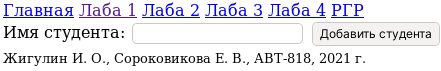
\includegraphics{before}
	\caption{Пустой список студентов}
\end{figure}

\begin{figure}[H]
	\centering
	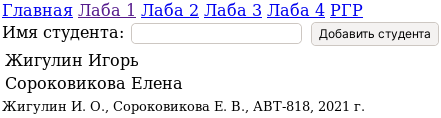
\includegraphics{after}
	\caption{Список студентов}
\end{figure}



\section{Вывод}
В ходе выполнения лабораторной работы бало разрабоано MVC приложение, которое позволяет просматривать и пополнять список студентов. Местом для хранения списка студентов была выбрана оперативная память. К достоинствам способа хранения можно отнести быстроту и простоту в использовании. Недостаток же заключается в том, что данные в оперативной памяти потеряются после перезапуска сервера.

\end{document}




